\chapter{Subvariedad 1-dimensional}
\section{Teorema de la funci\'on impl\'icita}
Este teorema es uno de aquellos que es dif\'icil de comprender por las
diferentes condiciones que se deben cumplir, del mismo modo, llega a 
varias conclusiones. Comenzaremos con un ejemplo.

\begin{example}\label{ex:unit-circle}
    Tenemos el c\'irculo unitario $x^{2} + y^{2} = 1$ con centro en el
    origen. Sabemos que  $x^{2} + y^{2} = 1$ no es una funci\'on ya que
    para cada $x$ en el dominio tenemos dos $f(x)$ en el rango, esto se
    puede ver claramente en la figura \ref{fig:unit-circle12} (a). 

    \begin{figure}[!ht]%
        \centering
        \subfloat[]{{\includegraphics[width=0.45\textwidth]{gfx/unit-circle1} }}%
        \label{fig:unit-circle123}
        \qquad
        \subfloat[]{{\includegraphics[width=0.45\textwidth]{gfx/unit-circle2} }}%
        \caption{C\'irculo unitario}
        \label{fig:unit-circle12}
    \end{figure}


    Pero si tomamos una vecindad de $x$ ( figura \ref{fig:unit-circle12} (b) )
    podemos definir la funci\'on $y = \sqrt{1-x^{2}}$ o $y = -\sqrt{1-x^{2}}$
    dependiendo de si $x$ esta por arriba o por abajo del eje-$x$. La
    pregunta ahora es ¿podemos hacer este mismo razonamiento para cualquier
    punto en el c\'irculo?. La respuesta es no. Si tomamos los puntos
    $(1,0)$ y $(-1,0)$ no podemos encontrar una vecindad lo suficientemente
    pequeña que cumpla que por cada $x$ tengamos un \'unico $f(x)$, ver
    figura \ref{fig:unit-circle3}.

    \begin{figure}[ht]
      \begin{center}
      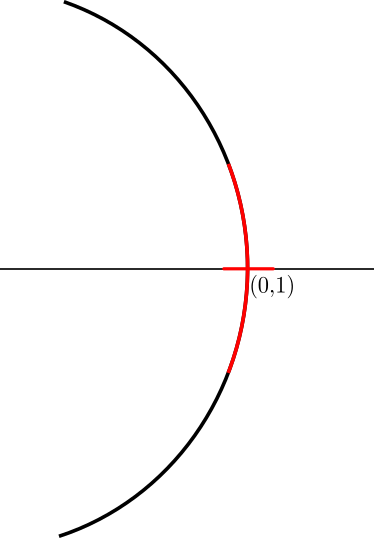
\includegraphics[width=0.5\linewidth]{gfx/unit-circle3}
        \caption{Punto cr\'itico}
      \label{fig:unit-circle3}
      \end{center}
    \end{figure}



    Hasta ahora tenemos que
    $$y = \sqrt{1-x^{2}} \text{,} \quad y = \sqrt{1-x^{2}}$$
    son dos funciones \emph{explicitas} que dan la misma relaci\'on que
    $x^{2} + y^{2} = 1$, de forma local para cada punto excepto 
    $(1,0)$ y $(-1,0)$.

    Entonces el teorema de la funci\'on impl\'icita provee condiciones
    bajo las cuales la relaci\'on de la forma $F(x,y)=0$ puede ser
    redefinida como una funci\'on $y=f(x)$ localmente.
\end{example}

Aunque no demostraremos este teorema, el siguiente ejemplo nos acerca a la
idea de su demostraci\'on para funciones de una o dos variables.

\begin{example}
    Tenemos la relaci\'on $y^{5}+y^{3}+y+x=0$.
\end{example}

    Vemos que es trivial definir $x=f(y)$, pero ahora la pregunta es ¿podemos
    definir $y=f(x)$?. La respuesta no es obvia, podriamos intentar resolver
    en terminos de $x$, pero, eso supone que podemos encontrar ra\'ices de 
    polinomios de grado 5, lo cual Galois demostró que no es posible. Tratemos
    ahora fijando $x$, por ejemplo en $x_{0}$, y definamos
    $$ \phi(y)=y^{5}+y^{3}+y+x_{0}$$
    entonces,
    $$\phi'(y)=5y^{4}+3y^{2}+1 > 0$$
    vemos que $\phi'(y)$ es estrictamente creciente en todo su dominio $\realR$,
    esto nos dice que $\phi(y)$ cruza el eje-x, es decir, $\phi(y)$ tiene exactamente
    una ra\'iz, sea $y_{0}$.

    Vemos que para cada $x$ tenemos una $y$ \'unica tal que $f(x)=0$, en otras
    palabras, encontramos una funci\'on $y=f(x)$, pero $f$ es \'implicita.

    Este teorema nos dice, entre otras cosas, que la relaci\'on $y=f(x)$
    existe pero no nos da una f\'ormula para encontrarla.

\clearpage

\begin{theorem}[Teorema de la funci\'on impl\'icita]
    Sea $\overrightarrow{x} = (x_{1},x_{2},\ldots,x_{n})$ y sea $F(\overrightarrow{x},y) \in C^{1}$ 
    en una vecindad de $N_{0}(\overrightarrow{x_{0}},y_{0})$ tal que
    \begin{enumerate}
        \item $F(N_{0}) = 0$
        \item $\frac{\partial F}{\partial y}(N_{0}) \ne 0$
    \end{enumerate}
    entonces existe una vecindad de $(N_{0})$ en donde existe una
    funci\'on \'implicita $y=f(\overrightarrow{x})$ tal que
    \begin{enumerate}[i.]
        \item $f(\overrightarrow{x_{0}}) = y_{0}$
        \item $F(\overrightarrow{x}, f(\overrightarrow{x})) = 0$
        \item $\frac{\partial f}{\partial x_{i}} = -\cfrac{\cfrac{\partial F}{\partial x_{i}}(\overrightarrow{x},f(\overrightarrow{x}))}{\cfrac{\partial F}{\partial y}(\overrightarrow{x},f(\overrightarrow{x}))}$
    \end{enumerate}
\end{theorem}

\subsection{Caso especial: curva}

Para una funci\'on dada $F$ de dos variables $x,y$ la ecuaci\'on $F(x,y) = 0$ describe
una curva siempre y cuando $\frac{\partial F}{\partial x} \ne 0$ o $\frac{\partial F}{\partial y} \ne 0$
en cada punto que satisfaga $F(x,y) = 0$. Si esto se cumple, entonces la curva puede ser
parametrizada localmente como una curva \emph{regular} parametrizada. Se dice que una curva 
es regular si su derivada no mapea al $0$.

La generalizaci\'on de este conc\'epto a la situaci\'on de varias variables y varias funciones
reales simultaneamente, nos da directa y naturalmente, la noci\'on de \emph{subvariedad}

\section{Subvariedad 1-dimensional}

\begin{definition}[Subvariedad]
    Una subvariedad k-dimensional (de clase $C^{\alpha}$) $M \subset \realR^{n}$ está definida por
    la condici\'on  de que $M$ est\'a dada localmente como el conjunto cero $F^{-1}(0)$ de un
    mapeo continuo ($\alpha$-veces) diferenciable
    $$ U \subset \realR^{n}  \xrightarrow{F} \realR^{n-k}$$
    con rango m\'aximo, es decir, $rank(J_{x}F|_{x})= n - k$ para cada $x \in M \cap U$, donde
    $M \cap U = F^{-1}(0)$ se cumple para una vecindad de $U$, para cada punto en $M$. \\
    Localmente, tambi\'en podemos describir a $M$ como la im\'agen de una inmersi\'on (ver
    definici\'on \ref{def:immersion}) de clase $C^{\infty}$
    $$ V \subset \realR^{k} \xrightarrow{f} M \subset \realR^{n} $$
    donde $rank(Df)=k$. Dicha $f$ es la parametrizaci\'on local, y $f^{-1}$ es llamada una \emph{carta}
    de $M$.
\end{definition}

Nuestro especial interes es cuando $k=1$, es decir, para una subvariedad 1-dimensional

\begin{definition}[Subvariedad 1-dimensional]
    Una subvariedad 1-dimensional (de clase $C^{\alpha}$) $C \subset \realR^{2}$ está definida por
    la condici\'on  de que $C$ est\'a dada localmente como el conjunto cero $F^{-1}(0)$ de un
    mapeo continuo ($\alpha$-veces) diferenciable
    $$ C \xrightarrow{F} \realR$$
    con $rank(J_{x}F|_{x})= 1$ para cada $x \in C$.
    \\
    Localmente, tambi\'en podemos describir a $C$ como la im\'agen de una inmersi\'on (ver
    definici\'on \ref{def:immersion})
    de clase
    $C^{\infty}$
    $$ I  \xrightarrow{f} C $$
    donde $rank(Df)=1$. Dicha $f$ es la parametrizaci\'on local, y $f^{-1}$ es llamada una \emph{carta}
    de $C$.
\end{definition}

En la definici\'on anterior, $C$ es la curva que estudiamos en el cap\'itulo 3.

\begin{example}
    En el ejemplo \ref{ex:unit-circle}, el c\'irculo unitario est\'a dado por la funci\'on
    $F(x,y)=x^{2}+y^{2}-1$. Vemos que $F$ es diferenciable,
    con
    $$ rank(J_{x}F|_{x})=rank((2x,2y))=1 $$
    entonces $F$ describe una subvariedad 1-dimensional.
\end{example}

\begin{example}
    En el ejemplo \ref{ex:unit-circle}, las funciones 
    $$y = \sqrt{1-x^{2}} \text{,} \quad y = -\sqrt{1-x^{2}}$$
    pueden parametrizarse
    $$ r(t)=(t,\sqrt{1-t^{2}}) \text{,} \quad c(t)=(t,-\sqrt{1-t^{2}}) $$
    respectivamente, de tal forma que $r^{-1}$ y $c^{-1}$ representan cartas
    de $C^{1}$ (circunferencia). Al conjunto $\{r^{-1}, c^{-1}\}$ se le llama
    un \emph{atlas} de $C^{1}$.
\end{example}

\begin{definition}[Espacio tangente a $\realR^{n}$]
    Para cada punto $x \in \realR^{n}$ el espacio
    $$ T_{x}\realR^{n} := \{x\} \times \realR^{n} $$
    es llamado el espacio tangente en el punto $x$ (el espacio de todos los vectores
    tangentes en el punto $x$). La derivada (o diferencial) $Df$ de un mapeo diferenciable
    $f$ esta definido como
    $$ Df|_{x}: T_{x}\realR^{k} \rightarrow T_{f(x)}\realR^{n} \quad \text{con} \quad
    (x,v) \mapsto (f(x),J_{x}f(v)) \text{.} $$
\end{definition}

\begin{definition}\label{def:immersion}
    Una inmersi\'on es un mapeo diferenciable entre subvariedades diferenciables donde su
    derivada es inyectiva. Explicitamente, $f:M \rightarrow N$ es una inmersi\'on si
    $$ D_{p}f: T_{p}M \rightarrow T_{f(p)}N $$
    es un mapeo inyectivo para toda $p \in M$. De forma equivalente, $f$ es una inmersi\'on
    si su derivada tiene rango igual a dim$M$:
    $$ rank D_{p}f = \text{dim}M \text{.} $$
\end{definition}

\begin{definition}[Espacio tangente a una subvariedad]
    Sea $M \subset \realR^{n}$ una variedad k-dimensional, y sea $p \in M$. El
    espacio tangente a $M$ en el punto $p$ es el subespacio vectorial $T_{p}M \subset T_{p}\realR^{n}$,
    el cual se define como
    $$ T_{p}M := Df_{u}(\{u\} \times \realR^{k})=Df_{u}(T_{u}\realR^{k}) $$
    para una parametrizaci\'on $f:U \rightarrow M$ con $f(u) = p$, donde $U \subset \realR^{k}$ es
    un conjunto abierto.
\end{definition}

\begin{example}
    En el caso en que $k=1$, tenemos que el espacio tangente $T_{p}C$ para una subvariedad 1-dimensional
    $C$ es
    $$ T_{p}C := Df_{u}(\{u\} \times \realR)=Df_{u}(T_{u}\realR) $$
    para una parametrizaci\'on $f$. Por simplicidad, se puede escribir $Df|_{x}: \realR \rightarrow \realR$
    cuando no hay peligro de confusi\'on. Entonces $Df|x$ se puede ver como mapeo
    ordinario entre espacios vectoriales, descritos \'unicamente por la matriz Jacobiana.
\end{example}

\begin{proposition}
    El espacio vectorial $T_{p}M$ es k-dimensional y no depende de la elecci\'on de $f$.
\end{proposition}
\begin{proof}
    Para probar esto, difinamos un difeomorfismo (ver definici\'on \ref{def:diffeomorphism}) $\phi: \realR^{k} \rightarrow M \subset \realR^{n}$,
    entonces tenemos que $\phi^{-1}$ es suave. Tenemos ahora un conjunto abierto $W \in \realR^{n}$ y
    un mapeo suave $\phi^{*}:\realR^{n} \rightarrow \realR^{k}$. Entonces $\phi^{*} \circ \phi$ es la
    identidad en $U$ y tenemos las siguientes transformaciones
    $$\realR^{k} \xrightarrow{D\phi} T_{x}(M) \xrightarrow{D\phi^{*}} \realR^{k} $$
    que describen el mapeo identidad en $\realR^{k}$. Se sigue que $D\phi:\realR^{k} \rightarrow T_{x}(M)$
    es un \emph{isomorfismo} (ver definici\'on \ref{def:isomorphism}), entonces dim$T_{x}(M)=k$. \qed
\end{proof}
